%!TEX root = ../clcxsj.tex

\chapter{线路要素计算程序设计}

\section{圆曲线与有缓和曲线的圆曲线}

\subsection{圆曲线的数学模型}

\begin{figure}[htbp]
    \centering
    \subfloat[左偏]
    {
        \label{fig:CircleRoute-Left}
        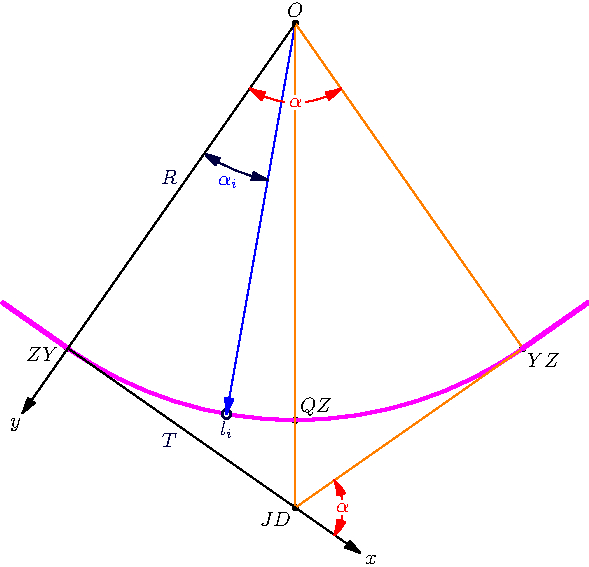
\includegraphics[scale=0.7]{route/LeftCircleRoute.pdf}
    }
    \hspace{1pt} %
    \subfloat[右偏]
    {
        \label{fig:CircleRoute-Right}
        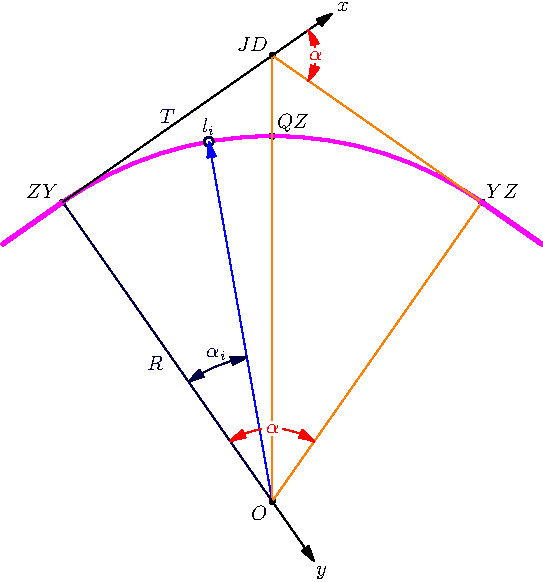
\includegraphics[scale=0.7]{route/RightCircleRoute.pdf}
    }
    \caption{圆曲线要素图}
    \label{fig:CircleRoute}
\end{figure}


% \begin{figure}[htbp]
%     \centering
%     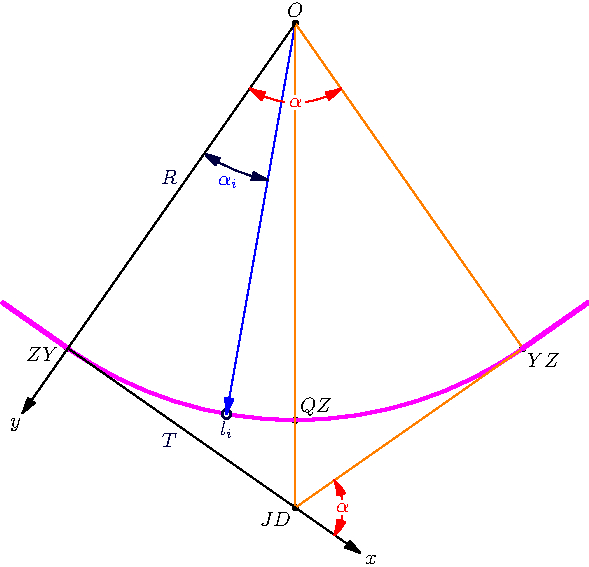
\includegraphics[scale=0.8]{route/LeftCircleRoute.pdf}
%     \caption{左偏-圆曲线要素图}
%     \label{fig:LeftCircleRoute}
% \end{figure}

% \begin{figure}[htbp]
%     \centering
%     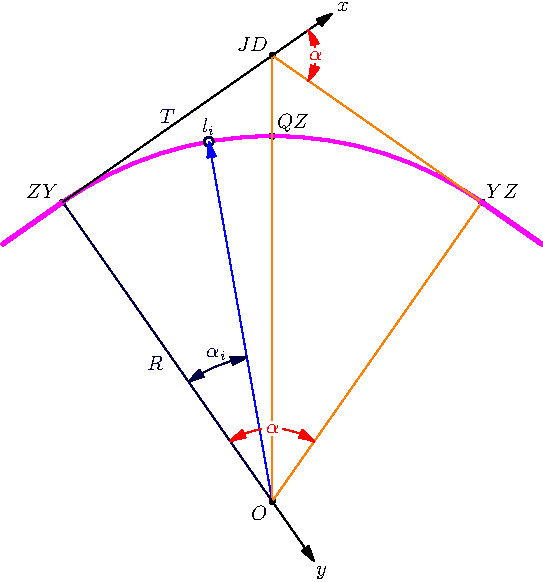
\includegraphics[scale=0.8]{route/RightCircleRoute.pdf}
%     \caption{右偏-圆曲线要素图}
%     \label{fig:RightCircleRoute}
% \end{figure}

 
 切线长:$T = R \cdot \tan (\alpha / 2)$

 曲线长:$L = R \cdot \alpha$

 外矢距:$E=R \cdot (\sec (\alpha /2) - 1)$

 切曲差:$q = 2T - L$

 \subsection{圆曲线上点的坐标计算}
 全站仪的坐标放样模式与GPS RTK可以十分方便的进行圆曲线上点的坐标放样。

 如图\ref{fig:CircleRoute}所示,以ZY点为原点,以ZY至JD切线方向为x轴,
 以ZY至O点方向为y轴建立ZY切线测量坐标系。从(a)与(b)两图可以看出
无论圆曲线是左偏还是右偏的,其坐标系是一致的。
 在ZY切线坐标系中用极坐标法按如下公式可以计算出圆曲线上任意一点$l_i$的坐标。

圆曲线偏左:

\begin{equation}
\left . 
\begin{aligned}
x_{i} &= R \sin \alpha_i   \\
y_{i} &= -R(1- \cos \alpha_i)
\end{aligned}
\right \}
\end{equation}

圆曲线偏右:

\begin{equation}
\left . 
\begin{aligned}
x_{i} &= R \sin \alpha_i   \\
y_{i} &= R(1- \cos \alpha_i)
\end{aligned} 
\right \}
\end{equation}

式中:$\alpha_i = l_i / R,  \alpha_i \le \alpha $, $l_i$可用圆曲线上任意一点的里程桩号
减去ZY点的里程桩号。

已知JD的坐标与里程桩号,根据圆曲线的结合几何要素$R, \alpha$即可计算出圆曲线上特征点的
里程桩号:

$KNo_{ZY} = KNo_{JD} - T$

$KNo_{QZ} = KNo_{ZY} + T/2$

$KNo_{YZ} = KNo_{QZ} + T/2$

在ZY切线坐标系中计算出圆曲线上各点的坐标之后,还需将其转换为测量坐标系
(或更正式的称为大地坐标系或独立施工坐标系)。在前一章我们已经做过坐标系的
转换了,在这个线路转换中,我们将ZY-JD边定义为x轴,因此两坐标系的夹角
即为ZY-JD边的坐标方位角,其转换关系如图\ref{fig:xytoxyroute}所示:

\begin{figure}[htbp]
    \centering
    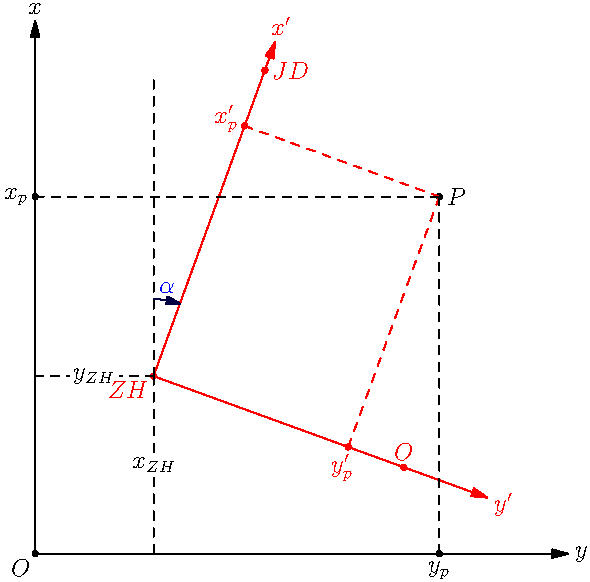
\includegraphics[scale=0.8]{route/xytoxyroute.pdf}
    \caption{ZY坐标系转测量坐标系}
    \label{fig:xytoxyroute}
\end{figure}

转换公式如下:

\begin{equation}
\left . \begin{aligned}
x_{P} &= x_{ZY} + x'_P \cos \alpha - y'_P \sin \alpha  \\
y_{P} &= y_{ZY} + x'_P \sin \alpha + y'_P \cos \alpha 
\end{aligned} \right \}
\label{eq:routexytoxy}
\end{equation}

 \subsection{缓和曲线的数学模型}

 \begin{figure}[htbp]
    \centering
    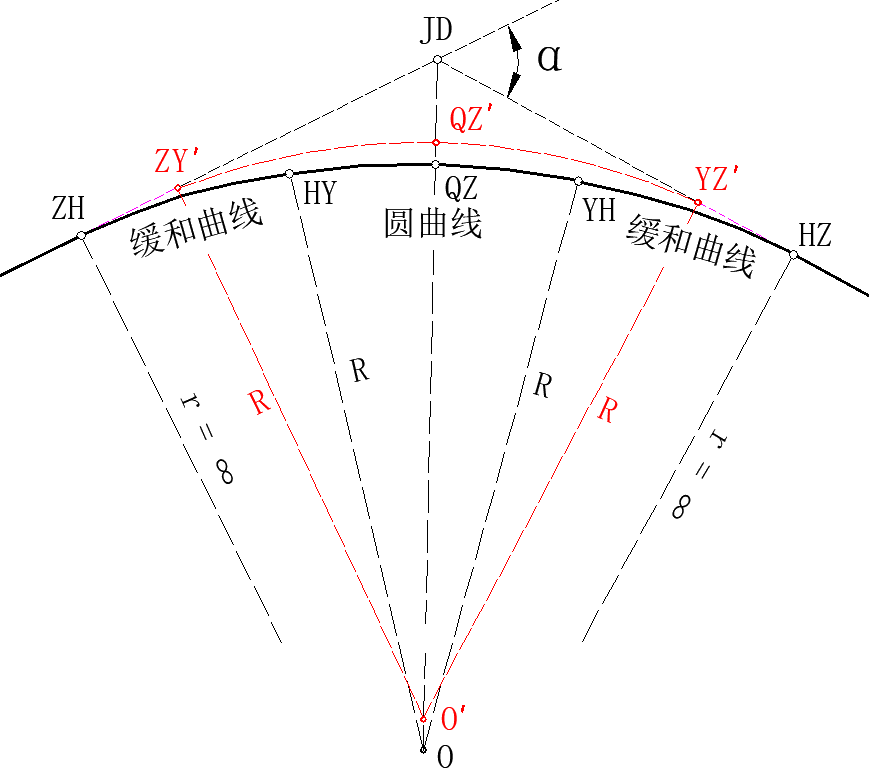
\includegraphics[scale=0.6]{route/HY01.png}
    \caption{缓和曲线的定义}
    \label{fig:HR01}
\end{figure}


\begin{figure}[htbp]
    \centering
    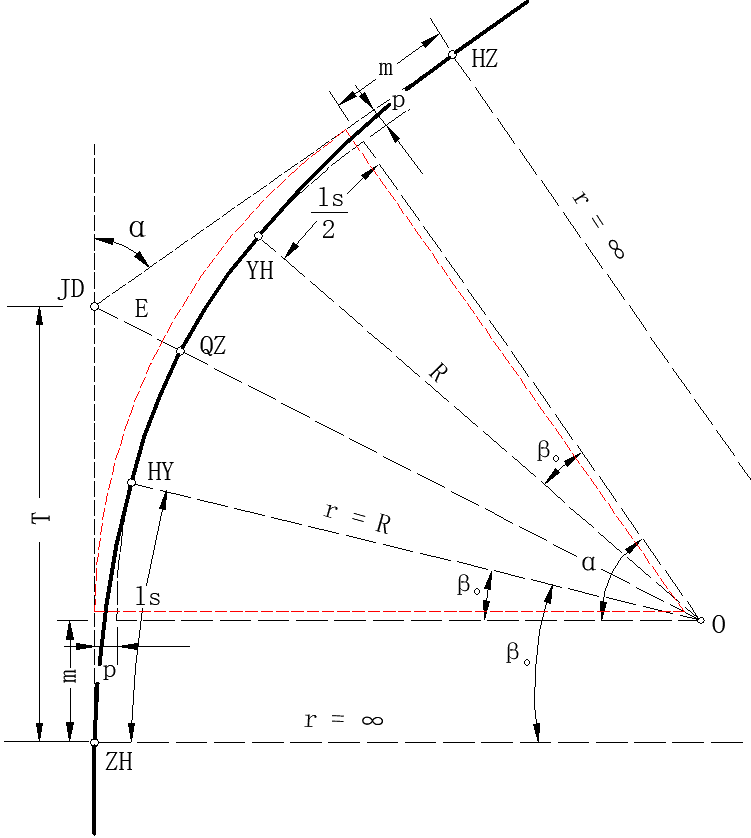
\includegraphics[scale=0.6]{route/HY02.png}
    \caption{缓和曲线的内移距和切线增长}
    \label{fig:HY02}
\end{figure}


\begin{figure}[htbp]
    \centering
    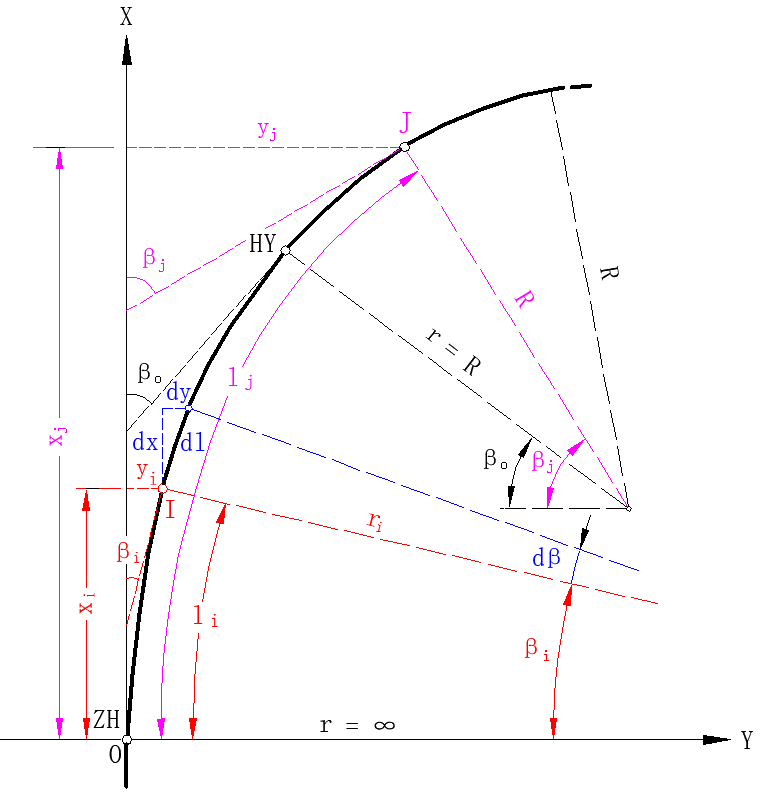
\includegraphics[scale=0.6]{route/HY03.png}
    \caption{缓和曲线的坐标计算}
    \label{fig:HR03}
\end{figure}

 缓和曲线参数计算公式为:

 $$\beta_0 = \frac{l_0}{2R} $$
切垂距:
$$m=\frac{l_0}{2} - \frac{l^3_0}{240R^2}$$
内移距:
$$p=\frac{l^2_0}{24R}$$

 
 切线长:$$T = m+ (R+p) \cdot \tan \frac{\alpha}{2}$$

 曲线全长:$$L = R \cdot (\alpha-2\beta_0)  + 2l_0$$

 圆曲线长:$$L_C = R \cdot (\alpha-2\beta_0)$$

 外矢距:$$E=(R+p) \cdot (\sec \frac{\alpha}{2} - 1)$$

\begin{enumerate}

\item  缓和曲线在ZH切线直角坐标系中的坐标计算(ZH段)

以ZH为坐标系原点,ZH至JD方向为x轴,过ZH点垂直于ZH-JD方向为y轴
建立坐标,如图\ref{fig:HY02}所示。则ZH部分缓和曲线上各点的坐标为:

\begin{equation}
\left .
\begin{aligned}
x_i &= l_i - \frac{l^5_i}{40R^2 l^2_0} + \frac{l^9_i}{3456R^4 l^4_0} - \frac{l^{13}_i}{599040R^6l^6_0} + ...  \\
y_i &=  \frac{l^3_i}{6Rl_0} - \frac{l^7_i}{336R^3 l^3_0} + \frac{l^{11}_i}{42240R^5l^5_0} -\frac{l^{15}_i}{9676800R^7l^7_0}+ ...  
\end{aligned} 
\right \}
\label{eq:routeZHXY}
\end{equation}

以上公式在计算中取前两项或前三项即可。

\item  缓圆点(HY)坐标计算公式为:

\begin{equation}
\left . \begin{aligned}
x_{HY} &= l_0 - \frac{l^3_0}{40R^2} + \frac{l^5_0}{3456R^4} - \frac{l^{7}_0}{599040R^6} + ...  \\
y_{HY} &=  \frac{l^2_0}{6R} - \frac{l^4_0}{336R^3} + \frac{l^{6}_i}{42240R^5} -\frac{l^{8}_0}{9676800R^7}+ ...  
\end{aligned} \right \}
\label{eq:routeHY}
\end{equation}

\item  圆曲线上点的坐标计算公式为:

\begin{equation}
\left . \begin{aligned}
x_{j} &= R \sin \beta_j + m \\
y_{j} &= R(1- \cos \beta_j) +p 
\end{aligned} \right \}
\label{eq:routeYQXY}
\end{equation}

\item  缓和曲线在HZ切线直角坐标系中的坐标计算(HZ段)

\begin{figure}[htbp]
    \centering
    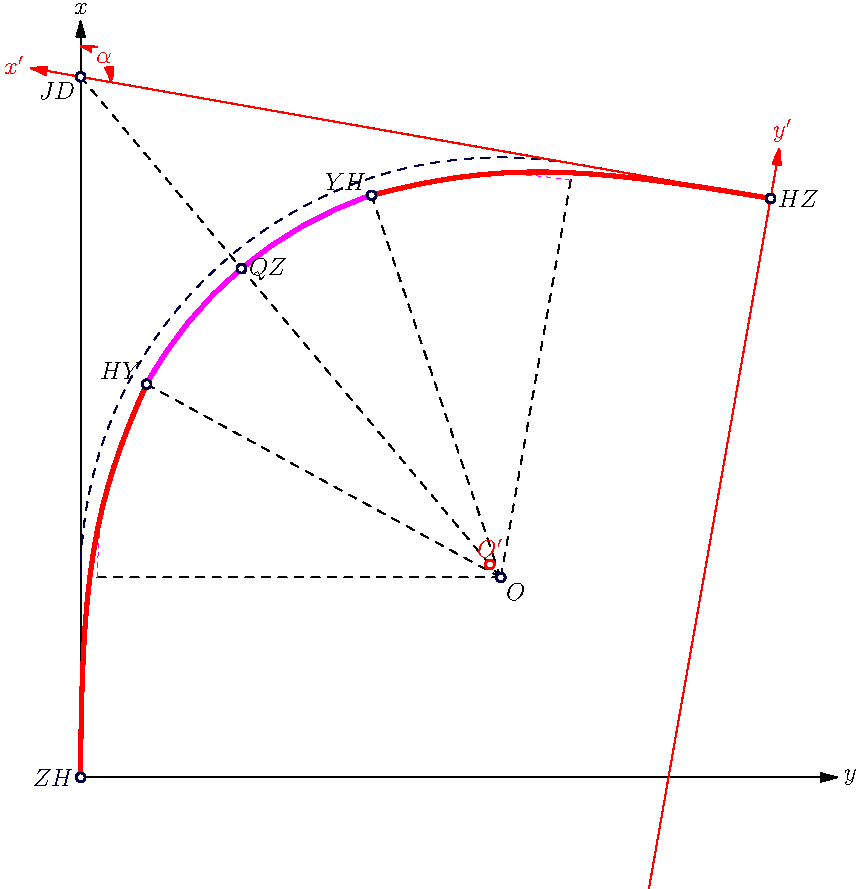
\includegraphics[scale=0.8]{route/RHY.pdf}
    \caption{缓和曲线的HZ部分坐标计算}
    \label{fig:RHY}
\end{figure}

如图\ref{fig:RHY}所示建立以缓直点HZ为原点,过HZ至JD方向为x轴,
过HZ点的缓和曲线切线为y轴的直角坐标系,计算另一半曲线任意一点的坐标$(x'_i, y'_i)$。
然后,将坐标转换为以ZH点为原点的直角坐标系中。

缓和曲线在HZ坐标系中的坐标可以先继续使用公式 \ref{eq:routeZHXY} 计算,然后由图\ref{fig:RHY}
可知将其转换为HZ坐标系中的坐标计算公式为:

\begin{equation}
\left . \begin{aligned}
x'_i &= x_i  \\
y'_i &= - y_i 
\end{aligned} \right \}
\label{eq:routeHZPtXY}
\end{equation}

为了将HZ坐标系中的点坐标转换为ZH坐标中,我们引用公式\ref{eq:routexytoxy}来计算,
请注意公式\ref{eq:routexytoxy}中的$\alpha$为$x'$轴的方位角(即x轴到$x'$轴的水平夹角),
因此图\ref{fig:RHY}应用到公式\ref{eq:routexytoxy}中的$\alpha$ 应为$\alpha + 180 \degree $。
如果将其代入公式\ref{eq:routexytoxy},则有转换公式为:

\begin{equation}
\left . \begin{aligned}
x_i &= x_{HZ} - x'_i  \cos \alpha + y'_i \sin \alpha \\
y_i &= y_{HZ}  -  x'_i \sin \alpha -  y'_i \cos \alpha 
\end{aligned} \right \}
\label{eq:routeHZtoZH}
\end{equation}

公式\ref{eq:routeHZtoZH}中的$(x_{HZ}, y_{HZ})$为HZ点在ZH坐标,其值为:

\begin{equation}
\left . \begin{aligned}
x_{HZ} &= T (1 +  \cos \alpha) \\
x_{HZ} &=  T \sin \alpha 
\end{aligned} \right \}
\label{eq:routeHZXY}
\end{equation}

也可以不用公式\ref{eq:routeHZtoZH},直接将$\alpha+180\degree$代入到
公式\ref{eq:routexytoxy}中进行计算。

在以上计算中,我们以曲线右偏为例的,如果曲线左偏,同样的方法建立坐标系,
x坐标是相同的, y坐标乘以 -1 即可。

\item 曲线上点坐标转换为大地坐标的计算公式为:

由于已经将曲线上的点坐标统一到ZH坐标系中了,我们继续引用公式\ref{eq:routexytoxy}
将ZH切线坐标系坐标转换到大地坐标系(测量坐标系)中,公式中的$\alpha$为$ZH \rightarrow JD$
的坐标方位角。

\end{enumerate}